\documentclass[a4paper]{article}

\usepackage{tikz}
\usepackage{pgfplots}
\usepackage{libertine}
\usetikzlibrary{patterns}

\pgfplotsset{compat=1.4} 
\pagestyle{empty}

\definecolor{bblack}{HTML}{111111}
\definecolor{wwhite}{HTML}{C8C8C8}

\makeatletter
\tikzset{nomorepostaction/.code=\let\tikz@postactions\pgfutil@empty}
\makeatother


\begin{document}

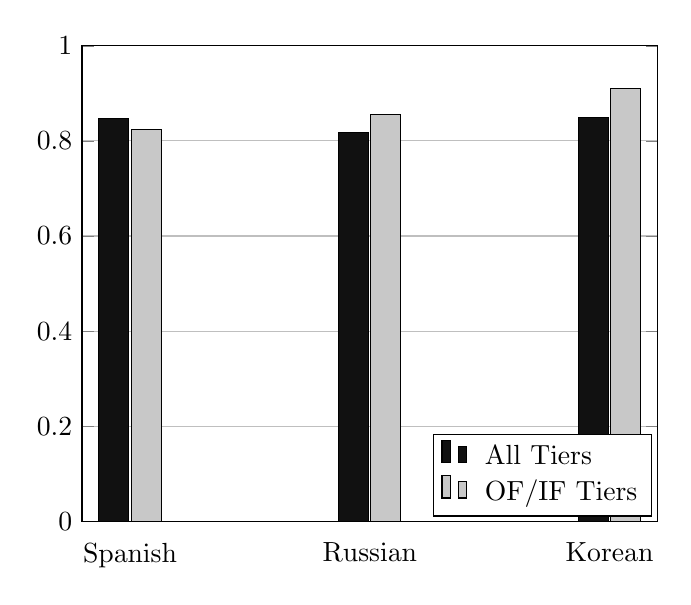
\begin{tikzpicture}
    \begin{axis}[
        width=3.5in,
	height=3in,
        major x tick style = transparent,
        ybar=2*\pgflinewidth,
        ymajorgrids = true,
        symbolic x coords={Spanish,Russian,Korean},
        xtick = data,
        scaled y ticks = false,
        enlarge x limits=0.1,
	ymin=0, ymax=1,
        legend cell align=left,
        legend style={
                at={(0.99,0.01)},
                anchor=south east,
                column sep=1ex
        }
    ]
  \addplot[style={bar width=0.15in,fill=bblack,draw=black}]
            coordinates {	(Spanish,0.8479)
				(Russian,0.8174)
				(Korean,0.8488)	    };
  \addplot[style={bar width=0.15in,fill=wwhite,draw=black}]
            coordinates {	(Spanish,0.8238)
				(Russian,0.8546)
				(Korean,0.9102)       };
 \legend{All Tiers,OF/IF Tiers}
 \end{axis}
\end{tikzpicture}
\end{document}

